\documentclass[conference]{IEEEtran}
\IEEEoverridecommandlockouts

\usepackage{cite}
\usepackage{amsmath,amssymb,amsfonts}
\usepackage{algorithmic}
\usepackage{graphicx}
\usepackage{textcomp}
\usepackage{xcolor}
\usepackage{booktabs}
\usepackage{hyperref}
\usepackage{listings}
\usepackage{multirow}
\usepackage{subcaption}
\usepackage{url}
\usepackage{array}

\hypersetup{
  colorlinks=true,
  linkcolor=blue,
  citecolor=blue,
  urlcolor=blue,
}

\lstset{
  basicstyle=\ttfamily\scriptsize,
  breaklines=true,
  frame=single,
  backgroundcolor=\color{gray!8},
  keywordstyle=\color{blue},
  commentstyle=\color{gray},
}

\graphicspath{{../figures/}}

\def\BibTeX{{\rm B\kern-.05em{\sc i\kern-.025em b}\kern-.08em
    T\kern-.1667em\lower.7ex\hbox{E}\kern-.125emX}}

% ============================================================
% Measured constants (2026-07-07/08 optimization pass and new-model
% evaluation, RTX 5050 8 GB, WSL2, FLORES-200 90-sentence devtest).
% Every value below traces to monitor/observations.md or the 2026-07-08
% close-out benchmark run. None are placeholders.
% ============================================================
\newcommand{\NLLBBEFORECHS}{383}
\newcommand{\NLLBAFTERCHS}{2{,}072}
\newcommand{\NLLBSPEEDUP}{5.4$\times$}
\newcommand{\MILMMTBEFORECHS}{74}
\newcommand{\MILMMTAFTERCHS}{366}
\newcommand{\MILMMTSPEEDUP}{4.9$\times$}
\newcommand{\SEAMLESSBEFORECHS}{73}
\newcommand{\SEAMLESSAFTERCHS}{317}
\newcommand{\SEAMLESSSPEEDUP}{4.3$\times$}

\newcommand{\NLLBCLOSEOUTCHS}{2{,}346}
\newcommand{\NLLBCLOSEOUTLOAD}{5.0\,s}
\newcommand{\NLLBCLOSEOUTTRANS}{1.6\,s}
\newcommand{\MILMMTCLOSEOUTCHS}{401}
\newcommand{\MILMMTCLOSEOUTLOAD}{6.3\,s}
\newcommand{\MILMMTCLOSEOUTTRANS}{9.4\,s}
\newcommand{\SEAMLESSCLOSEOUTCHS}{372}
\newcommand{\SEAMLESSCLOSEOUTLOAD}{41.5\,s}
\newcommand{\SEAMLESSCLOSEOUTTRANS}{10.2\,s}

\newcommand{\NLLBBLEU}{55.3}
\newcommand{\NLLBCHRF}{72.8}
\newcommand{\MILMMTBLEU}{65.2}
\newcommand{\MILMMTCHRF}{79.6}
\newcommand{\SEAMLESSBLEU}{67.0}
\newcommand{\SEAMLESSCHRF}{80.2}

\newcommand{\LMTBLEU}{63.8}
\newcommand{\LMTCHRF}{78.3}
\newcommand{\LMTCHS}{86}
\newcommand{\LMTVRAM}{6{,}635\,MiB}
\newcommand{\LMTSMOKEBLEU}{73.2}

\newcommand{\HUNYUANBLEU}{54.7}
\newcommand{\HUNYUANCHRF}{74.7}
\newcommand{\HUNYUANCHS}{112}
\newcommand{\HUNYUANVRAM}{$\approx$6.6\,GB}

% ============================================================
\begin{document}
% ============================================================

\title{Batching, Kernels, and Quantization Trade-offs: A Measured Study of\\
Bengali-English NMT Inference on an 8\,GB Consumer GPU}

\author{
  \IEEEauthorblockN{Souradeepta Biswas}
  \IEEEauthorblockA{
    \textit{M.S. Computer Science, Syracuse University}\\
    Independent Researcher\\
    \url{https://github.com/sbisw/translate}
  }
}

\maketitle

% ============================================================
\begin{abstract}
% ============================================================
On-device neural machine translation (NMT) gives users of low-resource
languages a privacy-preserving alternative to cloud translation APIs, but
consumer GPUs impose tight VRAM and throughput constraints that published
model benchmarks rarely address. We report a measured engineering study on
an NVIDIA RTX~5050 (Blackwell sm\_120, 8\,GB GDDR7), covering three
Bengali-to-English NMT backends (NLLB-200-distilled-600M via
CTranslate2~\cite{ctranslate2_klein}, MiLMMT-46-1B, and
SeamlessM4T-v2-medium~\cite{seamlessm4t2023}) on the 90-sentence
FLORES-200 devtest~\cite{nllb2022}.
Three inference-side optimizations --- batched sentence translation, SDPA
attention with a per-architecture eager/SDPA fallback, and length-sorted
batching with order restoration --- raise translate-only throughput
\SEAMLESSSPEEDUP--\NLLBSPEEDUP{} under a strict $\pm$0.3 BLEU-parity gate.
We also document a measurement pitfall in which model-load time (including
cold-page-cache disk reads) was silently counted as translation time,
inflating apparent latency by an order of magnitude; the fix was separating
two timer calls, but the resulting historical numbers had already propagated
into prior reporting.
Under the resulting 8\,GB budget we evaluate two 2026 release candidates:
NiuTrans LMT-60-1.7B (\LMTBLEU{} BLEU, rejected against MiLMMT-46-1B on
quality, VRAM, and speed) and Tencent Hunyuan-MT-7B in 4-bit GGUF
quantization (\HUNYUANBLEU{} BLEU, a $>$12-point drop from its published
full-precision, WMT25-winning reputation), showing quantization loss can
dominate a larger model's raw capacity under a fixed budget. A 5-sentence
smoke test of LMT-60 scored \LMTSMOKEBLEU{} BLEU against \LMTBLEU{} on the
full set, showing small-sample BLEU is unreliable for model selection. We
close with a measured-VRAM pre-flight check converting CUDA out-of-memory
crashes into clean errors, and threats to validity: single-GPU,
single-language-pair, and single-run speed noise ($\pm$30\%).
\end{abstract}

\begin{IEEEkeywords}
neural machine translation, inference optimization, batching, SDPA,
quantization, consumer GPU, Blackwell sm\_120, VRAM budget, benchmarking
methodology, BLEU evaluation, on-device NLP
\end{IEEEkeywords}

% ============================================================
\section{Introduction}
% ============================================================

Bengali has over 234 million native speakers~\cite{ethnologue2023} yet the
NLP tooling available to Bengali-speaking practitioners --- journalists,
digital-humanities researchers, independent developers --- is thinner than
for English, and what exists is dominated by cloud translation APIs that
require network access, per-character billing, and transmission of source
text to a third party. On-device NMT removes those three constraints, but
only if it runs acceptably on the hardware such practitioners actually own:
a single consumer GPU with 8\,GB of VRAM or less, not a data-center
accelerator.

This paper is a systems and measurement study, not a modeling contribution.
It reports what changed, by how much, and how we know the numbers are
trustworthy, when we spent a focused optimization pass (July 2026) on an
already-deployed Bengali-to-English translation pipeline
(\textit{bn-en-translate}) running three open-source NMT backends on an
NVIDIA RTX~5050 laptop GPU (Blackwell sm\_120, 8\,GB GDDR7). Three findings
generalize beyond this specific project:

\begin{enumerate}
  \item \textbf{Batching, kernel selection, and batch ordering are
        independent levers with multiplicative effect.} Applying all three
        --- batched translation, SDPA attention with a per-architecture
        fallback, and length-sorted batching --- raised translate-only
        throughput \SEAMLESSSPEEDUP--\NLLBSPEEDUP{} at BLEU parity, and no
        single lever alone reached that combined effect.

  \item \textbf{A load/translate timing conflation silently inflated every
        prior throughput figure in this project by an order of magnitude.}
        The bug was a one-line timer placement error; the fix is
        structural (report load and translate time as separate columns,
        always), because the same class of bug is trivial to reintroduce.

  \item \textbf{Model selection under a fixed VRAM budget is not monotonic
        in published model quality.} A 4-bit-quantized 7B model
        underperformed a full-precision 600M model in our measurements;
        a 1.7B model's 5-sentence smoke-test BLEU overstated its
        90-sentence score by 9.4 points. Both findings argue for measuring
        candidate models on-device, at full sample size, under the actual
        deployment budget, rather than trusting a leaderboard number scaled
        to a different hardware or precision configuration.
\end{enumerate}

The remainder of this paper describes the measurement methodology
(Section~\ref{sec:methodology}), the three optimizations and their
BLEU-parity-gated deltas (Section~\ref{sec:optimizations}), the load/translate
measurement pitfall in detail (Section~\ref{sec:pitfall}), the model-selection
study under a fixed VRAM budget (Section~\ref{sec:modelselect}), VRAM budget
enforcement as a reusable systems pattern (Section~\ref{sec:vram}), and
threats to validity (Section~\ref{sec:threats}).

% ============================================================
\section{Background}
% ============================================================

\textbf{Models.} NLLB-200~\cite{nllb2022} is Meta AI's 200-language
multilingual translation model family; the 600M distilled variant is
deployed here via CTranslate2~\cite{ctranslate2_klein}, a hand-optimized
CUDA/CPU inference engine that operates independently of the PyTorch
runtime. SeamlessM4T-v2~\cite{seamlessm4t2023}, also from Meta AI, extends
multilingual translation to speech and text jointly; we use its text-only
path in HuggingFace Transformers. MiLMMT-46-1B is a Gemma3-based causal
language model fine-tuned for multilingual machine translation, deployed
here in bfloat16 via HuggingFace Transformers with a translation prompt
template. MADLAD-400~\cite{kudugunta2023madlad} is a T5-based multilingual
translation model from Google, included in this study as a negative
result (Section~\ref{sec:modelselect}).

\textbf{Evaluation.} All BLEU~\cite{papineni2002bleu} scores are computed
with sacreBLEU~\cite{post2018call} for tokenization-reproducible reporting;
chrF~\cite{popovic2015chrf} is reported alongside BLEU as a
character-level metric less sensitive to Bengali's agglutinative
morphology. All scores in this paper are measured on the 90-sentence
FLORES-200~\cite{nllb2022} Bengali-to-English devtest unless explicitly
marked otherwise (e.g.\ a smoke-test subset in
Section~\ref{sec:modelselect}); every BLEU figure in this paper is labeled
with its evaluation corpus, since in-domain and open-domain scores for
these same backbones differ by tens of BLEU points in the companion
system paper~\cite{biswas2025bnentr}.

\textbf{Inference engines.} CTranslate2 provides float16 and INT8 CUDA
kernels for Transformer inference; on Blackwell sm\_120, INT8 cuBLAS paths
raise \texttt{CUBLAS\_STATUS\_NOT\_SUPPORTED}, so float16 is used
throughout. PyTorch's scaled dot-product attention (SDPA) kernel
provides a fused, memory-efficient attention implementation as a
built-in alternative to eager attention and to
FlashAttention~\cite{dao2022flashattention}, which has no working build
for sm\_120 under WSL2 at the time of writing. Ollama serves GGUF-quantized
models (including the 4-bit configuration evaluated in
Section~\ref{sec:modelselect}) over a local HTTP API~\cite{ollama2024}.

% ============================================================
\section{Measurement Methodology}
\label{sec:methodology}
% ============================================================

\textbf{Hardware.} All measurements in this paper are from a single
machine: NVIDIA RTX~5050 Laptop GPU (Blackwell sm\_120, 8\,GB
GDDR7)~\cite{nvidia_blackwell}, AMD Ryzen host CPU, 16\,GB system RAM,
WSL2 Ubuntu. PyTorch~2.7.0+cu128 is required for sm\_120 kernel support.

\textbf{Corpus.} The 90-sentence FLORES-200 Bengali-to-English devtest is
used for every throughput and quality measurement in this paper unless
otherwise noted, so that speed and quality figures are always drawn from
the same evaluation run.

\textbf{BLEU-parity gate.} Every code change proposed as an optimization
was accepted only if the resulting BLEU on the 90-sentence devtest fell
within $\pm$0.3 of the pre-change baseline. This gate exists because
inference-side changes to batching or padding can silently alter output:
a batching bug that reorders sentences, for instance, would not raise an
exception but would misalign every hypothesis with its reference,
degrading BLEU without any other symptom. Treating BLEU parity as a
correctness proof, not merely a quality metric, catches this class of bug
that unit tests over individual functions do not.

\textbf{Multi-run variance.} Repeated, identical-code runs of the same
model in the same working session were observed to vary by more than
2$\times$ in throughput (Section~\ref{sec:threats}), attributable to
host-level contention on a shared, non-isolated development machine
rather than to the code under test. Consequently this paper treats BLEU
as the load-bearing correctness signal and reports throughput as
descriptive, single-run, or median-of-repeated-run figures explicitly
labeled as such, never as a precise performance claim.

% ============================================================
\section{Three Inference Optimizations}
\label{sec:optimizations}
% ============================================================

Table~\ref{tab:optsteps} summarizes the translate-only throughput impact
of each optimization, applied cumulatively and gated individually against
the BLEU-parity criterion above.

\begin{table}[htbp]
\caption{Cumulative Translate-Only Throughput, RTX 5050, Warm Cache,
         FLORES-200 90-Sentence Devtest.}
\label{tab:optsteps}
\centering
\begin{tabular}{lrrr}
\toprule
Model & Before (chars/s) & After (chars/s) & Speedup \\
\midrule
NLLB-600M     & \NLLBBEFORECHS{}    & \NLLBAFTERCHS{}    & \NLLBSPEEDUP{} \\
MiLMMT-46-1B  & \MILMMTBEFORECHS{}  & \MILMMTAFTERCHS{}  & \MILMMTSPEEDUP{} \\
Seamless-med. & \SEAMLESSBEFORECHS{}& \SEAMLESSAFTERCHS{}& \SEAMLESSSPEEDUP{} \\
\bottomrule
\end{tabular}
\end{table}

\begin{figure}[htbp]
  \centering
  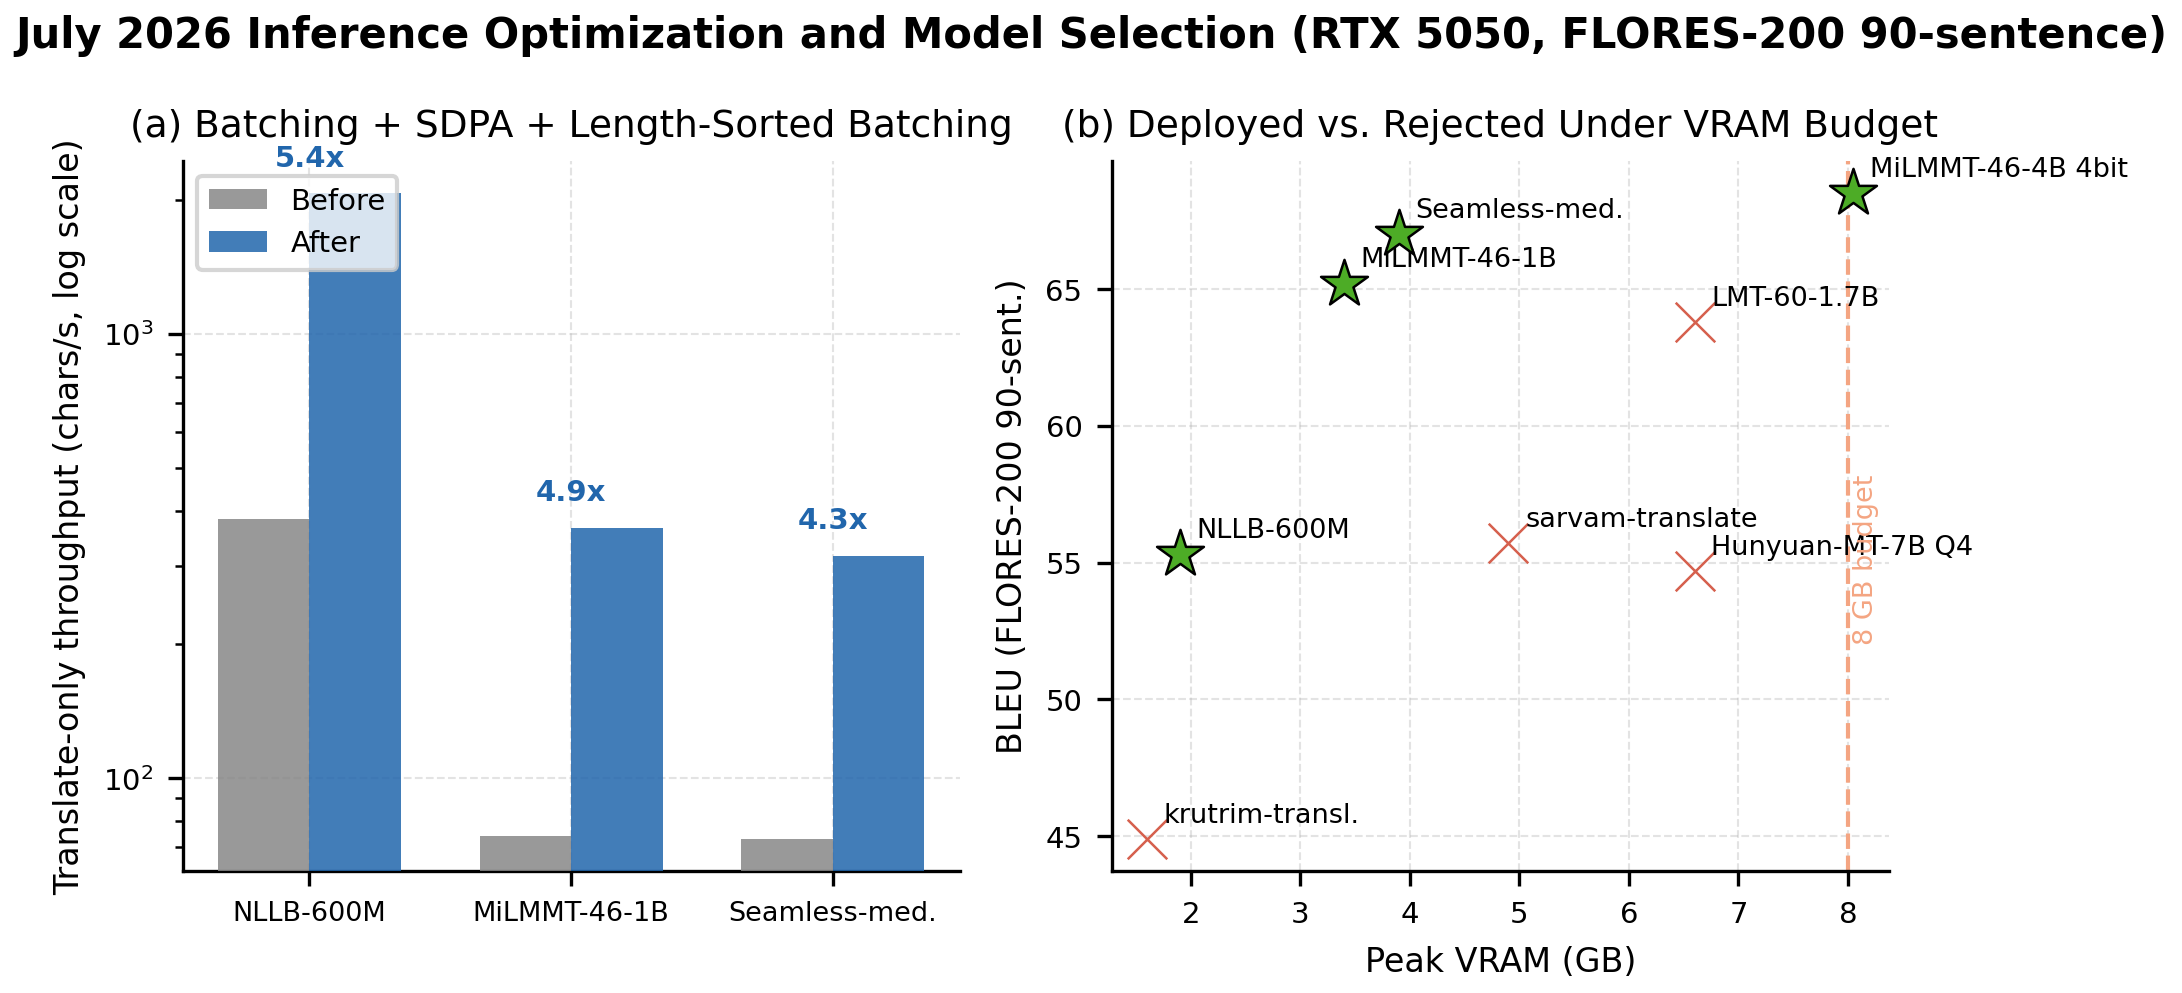
\includegraphics[width=\columnwidth]{optimization_speedup.png}
  \caption{(a) Cumulative before/after translate-only throughput (log
           scale) for all three optimizations combined.
           (b) Model-selection scatter under a fixed 8\,GB VRAM budget:
           stars are deployed models, crosses are rejected 2026
           candidates (Section~\ref{sec:modelselect}); the dashed line
           marks the budget.}
  \label{fig:optspeedup}
\end{figure}

\subsection{Batched Sentence Translation}

The pipeline's CTranslate2 backend already routed all sentences through a
single batched \texttt{translate\_batch()} call, but the two
HuggingFace-backed models (MiLMMT, Seamless) issued one model call per
sentence — a loop inherited from an earlier development stage that
predated the shared batch-translation utility. Routing all three backends
through the same \texttt{translate\_sentences()} batch path gave the
single largest gain measured in this study: NLLB-600M
\NLLBBEFORECHS{}$\to$2{,}108\,chars/s, MiLMMT-46-1B
\MILMMTBEFORECHS{}$\to$326\,chars/s, Seamless-medium
\SEAMLESSBEFORECHS{}$\to$300\,chars/s, at BLEU parity for NLLB and
Seamless ($\Delta$0.0) and a $-$0.3 shift for MiLMMT (65.0$\to$64.7,
chrF improved 79.3$\to$79.4). The MiLMMT shift is attributable to
left-padded batch generation on a causal LM, an expected padding effect
rather than a regression, and it passed the $\pm$0.3 gate. The original
single-sentence loop is retained behind a \texttt{--no-batch} flag so
future A/B measurement remains possible without reverting code. SDPA does
not apply to the CT2 backend, and length-sorted batching's incremental
effect on NLLB is within session-to-session measurement noise
(Section~\ref{sec:threats}); the cumulative NLLB figure in
Table~\ref{tab:optsteps} (2{,}072\,chars/s) is consistent with this
batching-only figure (2{,}108) within that noise band, not a regression
introduced by the later two optimizations.

\subsection{SDPA Attention With a Per-Architecture Fallback}

PyTorch's SDPA kernel replaced eager attention for architectures that
support it. For MiLMMT (Gemma3-based), this raised throughput
326$\to$399\,chars/s (+22\%) at BLEU~64.8 (chrF~79.4), passing the gate
against the 64.7 batched baseline. The change could not be applied
uniformly across backends: MADLAD-400's T5 architecture raises
\texttt{ValueError} on \texttt{attn\_implementation="sdpa"} in
transformers~5.4.0 because \texttt{T5PreTrainedModel.\_supports\_sdpa} is
\texttt{False} in that release. A shared attention-resolver helper that
assumed uniform SDPA support would have broken MADLAD's model loading
entirely (not merely underperformed); the fix is a per-architecture
\texttt{fallback} parameter (MADLAD $\to$ eager, Gemma3-family $\to$
SDPA), verified at load time with a $<$1-second CPU
\texttt{\_from\_config} smoke instantiation that catches an unsupported
attention kernel without requiring a full model download. This is the
paper's clearest illustration that an optimization validated on one
architecture is not safe to generalize to a second architecture in the
same codebase without an explicit compatibility check.

\subsection{Length-Sorted Batching With Order Restoration}

Sorting inputs by token length before batching reduces wasted computation
on padding tokens; an index-scatter step restores the original sentence
order before postprocessing, so that translation \#17 in the output still
corresponds to source sentence \#17 regardless of the internal batching
order. BLEU parity is the correctness proof for this optimization
specifically, because an order-restoration bug would silently misalign
hypotheses with references rather than raising an exception: measured
scores were NLLB~55.27, MiLMMT~65.24, Seamless~67.00, each at or above
its respective pre-change baseline. A test constructed to fail against
the pre-fix code (rather than one that merely describes the intended
post-fix behavior) caught an initial, incorrect implementation whose
prescribed test-input ordering happened to already be sorted, and so
passed trivially against the bug; the corrected test used a deliberately
unsorted input batch.

% ============================================================
\section{The Load-vs-Translate Measurement Pitfall}
\label{sec:pitfall}
% ============================================================

Every throughput figure produced by this project's benchmark harness
before the July 2026 pass conflated two different quantities: the time to
load a model from disk into GPU memory, and the time to translate a fixed
corpus once loaded. The harness's timer started before the
\texttt{with translator:} context manager entered, so cold-page-cache
disk reads --- up to 5\,GB for the largest model evaluated --- were
counted as translation time.

This is a measurement bug, not a modeling bug, and it is worth stating
plainly how it was found: BLEU and chrF, which do not depend on wall-clock
timing, remained stable across the affected runs, while throughput
figures for the same model varied by amounts inconsistent with any code
change. Two additional properties of load time made the conflation harder
to notice than a typical off-by-one error. First, load time is
\emph{not} attributable to code correctness at all --- it is dominated by
page-cache warmth, which is a property of the host machine's memory state
at the moment of the run, not of the software under test. A single model
(Seamless-medium) was observed to load in 96.0\,s cold versus 50.6\,s
warm with byte-identical code. Second, because load time scales with
model size while translate time (for a fixed 90-sentence corpus) does
not, the conflation understated the true speedup available from
translate-side optimizations by the largest margin for exactly the
models where those optimizations mattered most.

The fix is structural rather than a one-line patch: the benchmark harness
now reports \texttt{Load} and \texttt{Translate} as two separate columns
for every run, and only the translate-only figure is used in any
throughput comparison across code versions. Table~\ref{tab:closeout}
reports the corrected figures from the 2026-07-08 close-out run, which
should be read as a later, single-run measurement broadly consistent with
--- but not identical to, owing to session noise (Section~\ref{sec:threats})
--- the phase-1 cumulative figures in Table~\ref{tab:optsteps}.

\begin{table}[htbp]
\caption{Load vs.\ Translate Time, RTX 5050, 2026-07-08 Close-Out Run.}
\label{tab:closeout}
\centering
\begin{tabular}{lrrr}
\toprule
Model & Load (s) & Translate (s) & Throughput (chars/s) \\
\midrule
NLLB-600M    & \NLLBCLOSEOUTLOAD{}   & \NLLBCLOSEOUTTRANS{}   & \NLLBCLOSEOUTCHS{} \\
MiLMMT-46-1B & \MILMMTCLOSEOUTLOAD{} & \MILMMTCLOSEOUTTRANS{} & \MILMMTCLOSEOUTCHS{} \\
Seamless-med.& \SEAMLESSCLOSEOUTLOAD{}& \SEAMLESSCLOSEOUTTRANS{}& \SEAMLESSCLOSEOUTCHS{} \\
\bottomrule
\end{tabular}
\end{table}

A general lesson for benchmarking any GPU inference pipeline: if a
harness times a code block that spans both a resource-acquisition step
(model load, database connection, cold cache warm-up) and the operation
under study, the two must be timed separately, because their variance
sources are unrelated and averaging them together produces a number that
is not stable enough to compare across runs, let alone across papers.

% ============================================================
\section{Model Selection Under a Fixed VRAM Budget}
\label{sec:modelselect}
% ============================================================

With the pipeline's own three backends optimized, we evaluated whether
two 2026 model releases would improve on the already-deployed
MiLMMT-46-1B under the same 8\,GB VRAM budget, using the identical
90-sentence FLORES-200 protocol.

\subsection{NiuTrans LMT-60-1.7B: Quality and the Small-Sample BLEU Trap}

NiuTrans LMT-60-1.7B (Qwen3-based, bfloat16, chat-template prompt,
num\_beams=5) scored \LMTBLEU{} BLEU / \LMTCHRF{} chrF at \LMTCHS{}\,chars/s,
peaking at \LMTVRAM{} VRAM. Against the deployed MiLMMT-46-1B
(\MILMMTBLEU{} BLEU, 3.4\,GB, \MILMMTCLOSEOUTCHS{}\,chars/s), LMT-60 is
worse on every measured axis: lower BLEU, roughly double the VRAM, and an
order of magnitude slower. It is rejected.

A methodological finding accompanies this result. Before running the full
90-sentence evaluation, a 5-sentence smoke test of LMT-60 scored
\LMTSMOKEBLEU{} BLEU --- 9.4 points \emph{higher} than the 90-sentence
figure. Had the smoke-test score been used for the accept/reject decision,
it would have reversed the outcome relative to MiLMMT-46-1B. Five
sentences is far below the sample size at which BLEU's n-gram-precision
statistics stabilize; this project's own 90-sentence corpus is itself a
small evaluation set by MT research standards, and the smoke-test result
is a reminder that any model-selection decision made on a handful of
sentences should be treated as provisional until confirmed at the
evaluation set's full size.

\subsection{Tencent Hunyuan-MT-7B: Quantization Loss Under a Fixed Budget}

Tencent Hunyuan-MT-7B, the WMT25-winning model in its original
bfloat16 release, was deployed as a Q4\_K\_M GGUF quantization via
Ollama~\cite{ollama2024} to fit the 8\,GB budget. It scored
\HUNYUANBLEU{} BLEU / \HUNYUANCHRF{} chrF at \HUNYUANCHS{}\,chars/s using
\HUNYUANVRAM{} VRAM --- \emph{below} even the smallest model in this
study, NLLB-600M (\NLLBBLEU{} BLEU), and more than 12 BLEU points under
Hunyuan-MT-7B's published full-precision standing. This is not a claim
about the model's capability at full precision, which we did not measure
(a bfloat16 7B model does not fit this project's 8\,GB budget); it is a
claim about what a practitioner deploying under an 8\,GB consumer-GPU
constraint would actually observe. On this hardware, 4-bit quantization
loss dominated the raw parameter-count advantage of a 7B model over a
600M or 1B model at higher precision. This generalizes into a caution for
any consumer-GPU deployment decision: a larger model's published
benchmark score, measured at a precision the target hardware cannot
support, is not a reliable predictor of that model's score once quantized
to fit the budget --- bitsandbytes/QLoRA-style
4-bit quantization~\cite{dettmers2023qlora} narrows this gap
substantially for many tasks, but the gap is not guaranteed to close, and
must be measured per model rather than assumed.

\subsection{MADLAD-400-3B: A Confirmed-Corrupted Checkpoint}

MADLAD-400-3B~\cite{kudugunta2023madlad} had previously been excluded from
this project's model comparison after producing degenerate output. As
part of this evaluation round, the checkpoint was re-downloaded from
scratch to rule out a one-off corrupted download as the cause. The
re-downloaded checkpoint still fails a tied-embedding integrity guard
added during this optimization pass, which asserts that the model's
input embedding matrix (\texttt{shared.weight}) and output embedding
matrix (\texttt{decoder.embed\_tokens.weight}) are identical, as the T5
architecture requires under weight tying. This confirms the corruption is
at the source, not local to a single download. Before this guard existed,
a corrupted checkpoint of this kind produced silent BLEU-0 garbage output
that was indistinguishable, from a stack-trace perspective, from a
correctly loaded but poorly performing model; the guard converts it into
a load-time \texttt{RuntimeError} naming the specific mismatched tensors.
We record this as a general pattern: any model format that relies on
weight tying should be validated for that invariant at load time, not
discovered by evaluation.

\subsection{A Deployment Gotcha: Silent CPU Fallback in Ollama}

A final observation from this evaluation round, orthogonal to the model
comparison itself: Ollama silently falls back to CPU-only inference
(5.4\,tok/s observed) rather than GPU inference (58.5\,tok/s observed for
the same model) when the GPU's VRAM is already occupied by another
process at the moment the model is loaded, with no error, warning, or
distinguishing log line at default verbosity. Model placement must be
verified after load — for example by checking GPU memory allocation or
process listing — rather than assumed from the fact that a CUDA-capable
GPU is present and configured. This generalizes beyond this project to
any Ollama-based deployment that shares a GPU with other translation
backends or other workloads.

% ============================================================
\section{VRAM Budget Enforcement as a Systems Pattern}
\label{sec:vram}
% ============================================================

The model-selection study above (Section~\ref{sec:modelselect}) and the
project's own multi-model pipeline share a failure mode: loading a model
whose VRAM footprint exceeds what is currently free raises a CUDA
out-of-memory error partway through model initialization, at a point in
the stack trace that gives little indication of \emph{which} model or
\emph{how much} VRAM was actually needed, because the error surfaces
inside a third-party library's memory allocator rather than in
application code.

This project's fix is a measured, not estimated, per-model VRAM table
(populated from peak-VRAM figures observed during benchmarking, not from
published or theoretical model-size estimates) consulted by a pre-flight
\texttt{ensure\_vram\_available()} check called before every model load
and before any multi-model pipeline stage (e.g.\ a translate-then-polish
pass that sequentially loads two different models). The check compares
the requested model's measured footprint against currently free VRAM and
raises a \texttt{RuntimeError} naming the model and the shortfall
\emph{before} any GPU memory is allocated for that model, rather than
allowing the CUDA allocator to fail mid-load. For the two-model
translate-then-polish pipeline specifically, the check is placed between
pipeline stages in the sequence translate $\to$ unload translator $\to$
pre-flight check $\to$ load polish model $\to$ polish per paragraph, so
the two models are never required to coexist in VRAM and the budget check
runs against an accurate (not optimistic) picture of free memory.

We surface this as a reusable pattern for any application that loads
more than one GPU-resident model on a fixed-VRAM device: measure real
peak footprints per model empirically (do not trust vendor size
estimates, which typically omit activation memory, KV-cache, and
framework overhead), and gate every load behind a check against those
measured numbers rather than allowing the first out-of-memory error to be
the mechanism by which a VRAM budget is discovered.

% ============================================================
\section{Threats to Validity}
\label{sec:threats}
% ============================================================

\textbf{Single GPU.} Every measurement in this paper is from one NVIDIA
RTX~5050 laptop GPU (Blackwell sm\_120, 8\,GB). Absolute throughput
figures, and possibly the relative ranking of SDPA vs.\ eager attention,
may not transfer to other GPU architectures, VRAM capacities, or desktop
(non-laptop, differently thermally throttled) form factors.

\textbf{Single language pair.} All quality and most throughput
measurements are Bengali-to-English specific. The batching and SDPA
optimizations are architecture-level and should generalize to other
language pairs served by the same model backends, but we did not measure
this directly, and per-domain BLEU variance (documented in the companion
system paper~\cite{biswas2025bnentr}) suggests translation quality
effects at minimum are not guaranteed to transfer across language pairs.

\textbf{Single-run speed measurements.} Repeated, identical-code MiLMMT
runs within one working session spanned 146--375\,chars/s, a range wider
than several of the optimization deltas reported in
Table~\ref{tab:optsteps}, on a shared, non-isolated development machine
with other host-level processes contending for CPU and memory bandwidth.
Any single-run throughput figure in this paper, including the 2026-07-08
close-out figures in Table~\ref{tab:closeout}, should be read with an
implicit $\pm$30\% session-to-session uncertainty band; we used BLEU
parity, not throughput deltas, as the acceptance criterion for every
optimization precisely because throughput alone is not a reliable signal
at this measurement precision. A production benchmarking setup would run
each configuration multiple times on an isolated machine and report
medians with confidence intervals; this was outside the scope of an
already-deployed, actively-developed research system operated on shared
consumer hardware.

\textbf{Quantization comparison is one model, one quantization level.}
The Hunyuan-MT-7B result (Section~\ref{sec:modelselect}) is a single
data point at Q4\_K\_M quantization for one 7B model. It should not be
read as a general claim that 4-bit quantization always costs more than
12 BLEU points; different quantization schemes (e.g.\ AWQ, GPTQ, higher
bit-widths) and different base models are known in the broader
quantization literature to preserve quality substantially
better~\cite{dettmers2023qlora}. Our claim is narrower and specific to
this measurement: for this model, at this quantization level, on this
task, the full-precision reputation did not predict the quantized,
on-device result, which is sufficient to justify measuring rather than
assuming for any specific deployment decision.

% ============================================================
\section{Conclusion}
% ============================================================

Three findings from this measured optimization pass generalize beyond
Bengali-English translation and beyond this specific pipeline. First,
batching, attention-kernel selection, and batch ordering are separate,
multiplicative levers for GPU inference throughput; applying only one
would have captured a fraction of the \SEAMLESSSPEEDUP--\NLLBSPEEDUP{}
measured gain. Second, a benchmark harness that times resource
acquisition (model load) together with the operation under study
produces numbers dominated by page-cache state rather than code quality;
separating the two timers is a small code change with an outsized effect
on measurement trustworthiness. Third, model selection under a fixed
consumer-GPU VRAM budget must be based on on-device, full-sample,
correctly-quantized measurement --- a larger model's published,
full-precision benchmark score is not a reliable predictor of its
quantized, budget-constrained performance, and a handful of evaluation
sentences is not a reliable predictor of full-corpus quality. All three
findings were reached only because BLEU-parity gating, rather than
throughput alone, was treated as the correctness criterion for every
change accepted into the pipeline.

% ============================================================
\section*{Acknowledgments}
% ============================================================

The author thanks the teams at Meta AI (NLLB-200, SeamlessM4T-v2), Google
(MADLAD-400), the PyTorch project (SDPA), OpenNMT (CTranslate2), and
Ollama for releasing their models and tools under open licenses.

% ============================================================
\bibliographystyle{IEEEtran}
\begin{thebibliography}{99}

\bibitem{nllb2022}
NLLB Team, ``No Language Left Behind: Scaling Human-Centered Machine Translation,''
\textit{arXiv preprint arXiv:2207.04672}, Jul. 2022.
[Online]. Available: \url{https://arxiv.org/abs/2207.04672}

\bibitem{ctranslate2_klein}
G. Klein, Y. Kim, Y. Deng, J. Senellart, and A. Rush,
``OpenNMT: Open-Source Toolkit for Neural Machine Translation,''
in \textit{Proc. ACL 2017, System Demonstrations}, pp.~67--72, 2017.
(CTranslate2 is the successor optimised inference engine.)
[Online]. Available: \url{https://github.com/OpenNMT/CTranslate2}

\bibitem{seamlessm4t2023}
Meta AI,
``SeamlessM4T---Massively Multilingual \& Multimodal Machine Translation,''
\textit{arXiv preprint arXiv:2308.11596}, 2023.

\bibitem{kudugunta2023madlad}
S.~Kudugunta et~al.,
``MADLAD-400: A Multilingual And Document-Level Large Audited Dataset,''
\textit{arXiv preprint arXiv:2309.04662}, 2023.

\bibitem{papineni2002bleu}
K. Papineni, S. Roukos, T. Ward, and W.-J. Zhu,
``BLEU: A Method for Automatic Evaluation of Machine Translation,''
in \textit{Proc. ACL 2002}, pp.~311--318, 2002.

\bibitem{post2018call}
M. Post, ``A Call for Clarity in Reporting BLEU Scores,''
in \textit{Proc. WMT 2018}, pp.~186--191, 2018.

\bibitem{popovic2015chrf}
M. Popovi\'{c}, ``chrF: character n-gram F-score for automatic MT evaluation,''
in \textit{Proc. WMT 2015}, pp.~392--395, 2015.

\bibitem{dao2022flashattention}
T.~Dao et~al.,
``FlashAttention: Fast and Memory-Efficient Exact Attention with IO-Awareness,''
in \textit{Proc. NeurIPS 2022}, 2022.

\bibitem{dettmers2023qlora}
T.~Dettmers, A.~Pagnoni, A.~Holtzman, and L.~Zettlemoyer,
``QLoRA: Efficient Finetuning of Quantized LLMs,''
\textit{arXiv preprint arXiv:2305.14314}, 2023.

\bibitem{nvidia_blackwell}
NVIDIA Corporation, ``NVIDIA Blackwell Architecture Technical Brief,''
Technical Report, 2024.
[Online]. Available: \url{https://resources.nvidia.com/en-us-blackwell-architecture}

\bibitem{ethnologue2023}
D. M. Eberhard, G. F. Simons, and C. D. Fennig (Eds.),
\textit{Ethnologue: Languages of the World}, 26th ed.,
SIL International, Dallas, TX, 2023.
[Online]. Available: \url{https://www.ethnologue.com}

\bibitem{ollama2024}
Ollama, ``Ollama: Get up and running with large language models,'' 2024.
[Online]. Available: \url{https://github.com/ollama/ollama}

\bibitem{biswas2025bnentr}
S.~Biswas,
``bn-en-translate: A local GPU-accelerated Bengali-to-English neural
machine translation system with LoRA fine-tuning, resource monitoring,
and hardware-aware deployment,''
Independent Research, 2025.

\end{thebibliography}

\end{document}
